\chapter{Introduction}

\section{Motivation}

For a long time the speed of programs experienced a constant growth through improved processor hardware. Intel co-founder Gordon E. Moore was one of the first persons to describe this trend in 1965. This description is well known by the name Moore's law which initially stated that the number of transistors on an integrated circuit doubles every year \cite{moore_law}. This trend slowed down and Moore had to change the interval to two years a decade later \cite{moore_law_2003}. The most important consequence however has been realized by one of Moore's co-workers at Intel, David House, who predicted that the performance of processors would double every 18 months \cite{moore_law_2003}. As a result, an increase in computing power could be obtained simply by running the same programs on newer hardware. As a consequence, hardware dominated the growth of programs' performance for a long period of time.

Unfortunately, processing hardware technologies hit a limit at the beginning of the third millennium. Physical bounds, like the size of atoms, prevented a further shrinking of integrated circuits which would allow an increase in clock speed. Therefore, processor vendors like Intel and AMD started to place multiple CPUs on a single chip which still lead to an increase in computational power but in a different way than in the last 40 years. This change is sometimes referred to as the multicore crisis \cite{multicore_crisis}. The consequence from a software developer's perspective is that traditional algorithms stopped gaining speed by being run on newer hardware. In fact, improving performance is now up to the programmer, who is responsible for writing concurrent and parallel software that can make full use of the underlying hardware's capabilities. 

But multicores were not the only major hardware change that had an impact on the way software is developed recently. Graphics cards, which were initially intended to offload and accelerate 2D and 3D graphic operations from the CPU to a separate hardware device, started to gain popularity in non graphical areas of programming. A GPUs intense floating point processing power and parallel nature by design makes it ideal for uses in several areas of science, business and engineering (General Purpose GPU). When used in the right place, a GPU may compute results several magnitudes faster than the CPU \cite{gpu_history}. However, due to the very different hardware architecture, the graphics card is still not suitable to efficiently solve the same problems as a CPU does.

Todays software engineers working in performance focused domains have a hard time designing their applications. With two different types of processors (CPU and GPU), both excellent in their own ways, and a lot of APIs and frameworks around them (OpenMP, CUDA, OpenCL, DirectCompute, C++ AMP, ...), the available hardware and corresponding software is more heterogeneous than ever. Thus, profound knowledge of the available technologies, their performance and restrictions as well as the consequences for a development team is essential for choosing the optimal strategy to tackle todays computational needs.

\section{Goal}
The goal of this thesis is to provide the reader with a state of the art comparison of modern GPU and CPU performance in solving traditional problems such as sorting arrays and multiplying matrices using various approaches.
The GPU algorithms will be implemented using the Open Computing Language (OpenCL). Therefore the reader is given a short introduction into OpenCL in order to understand the provided code samples and how programming for a GPU works. These OpenCL implementations are benchmarked against algorithms implemented in C/C++ solving the same problem. It is important to note that the GPU and CPU version do not necessarily have to use the same algorithm, they only have to output the same result. This decision was inevitable due to the highly diverse hardware properties of the CPU and the GPU.
The problems chosen for this comparison are sorting an array, multiplying two large matrices and calculating the parallel prefix sum of an array (explained in corresponding chapter \ref{sec:prefix_sum}). These algorithms cover several different aspects that play an important role when implementing software for a GPU such as runtime complexity, memory footprint and memory transfer time vs. computation time. 

Eventually, the results of benchmarking the chosen algorithms should give the reader an idea of how much a GPU can accelerate different kinds of algorithms and what a programmer has to pay attention to when developing GPGPU accelerated software. This knowledge is not only valuable during developing but also useful when choosing the right technology for a given problem. This thesis should aid all software engineers in understanding how GPU computing works and where it should be used.

\section{History of GPGPU Computing} 
\label{sec:history}
Before we go into details about OpenCL and several GPU implementations, some background information about how GPUs have evolved is provided which may help understanding the design and peculiarities of graphics hardware. The following information is taken from a paper survey in 2010 \cite{gpu_history}.

In the early 1980's a "GPU" was nothing more than an integrated frame buffer, an additional chip that relied on the CPU for drawing.

One of the first dedicated video cards was the IBM Professional Graphics Controller (PGA) released in 1984. It used an on-board Intel 8088 microprocessor to take care of graphical calculations in order to take off load from the main processor (CPU). Although the Intel 8088 was in fact a conventional CPU, the PGA's separate on-board processing unit marked an important step towards the development of GPUs as co-processors.

In the following years more graphics orientated features where added like shading, lighting, rasterization, the depth buffer and color blending. With the introduction of OpenGL in 1989 by Silicon Graphics Inc. (SGI), the world's first application programming interface (API) for 2D and 3D graphics was released. OpenGL was designed upon a concept called the graphics pipeline which depicts video processing as data traveling through multiple stages of operations. The pipeline begins at the CPU by sending geometry data together with colors, textures etc., which is then transformed from the initial 3D coordinate space to pixel coordinates. Lighting operations use material colors and textures to shade the incoming triangles which are then rasterized into the frame buffer for display. As the programmer was not able to alter the functionality if the pipeline it is also well known under the term "fixed function pipeline". This processing model determined the design of graphics hardware for more then a decade.

In the mid 1990's NVIDIA, ATI and Matrox started to provide graphic controllers for consumers. Famous computer games like Quake and Doom became popular spurring the gaming industry and the interest in GPUs. However, GPUs at this time were only able to output one pixel per clock cycle and CPUs were able to send more triangles than the GPU could handle. This problem lead graphic hardware vendors to adding more pipelines and eventually more cores to their GPUs in order to enable parallel pixel processing and increase the throughput.

NVIDIA's release of the GeForce 3 in 2001 marked an important step in the evolution of GPUs by loosening the restrictions of the fixed function pipeline. With the ability of writing small programs for the GPU, which could operate on the vertices traveling through the pipeline, programmers were given a tool to make limited changes to the behavior of the pipeline. These programs were called vertex shaders and were written in an assembly-like language. One year later the pixel shader followed running on a separate part of the GPU hardware.

\begin{figure} % from http://wiki.ega.org.pl/images/b/b4/Pipeline.png
\centering
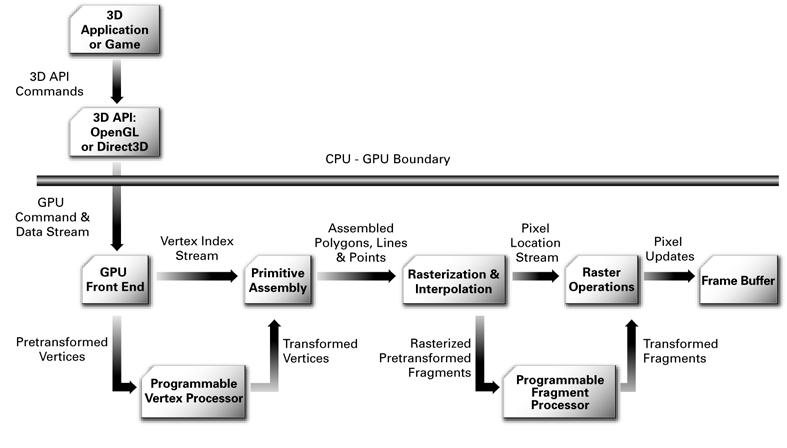
\includegraphics[width=0.7\linewidth]{pipeline2}
\caption{The graphics pipeline with programmable vertex and fragment processor. \cite{cg_book}}
\label{fig:pipeline2}
\end{figure}

With the introduction of the High Level Shading Language (HLSL) with DirectX 9 in 2003 programming GPU hardware became easier than with the previous shaders written in assembler. The first developers started to use the available programmability for non-graphical tasks. The first attempts of GPU computing emerged. A year later in 2004 Brook and Sh appeared representing the first languages targeting GPGPU computing.
Although the workflow of the GPU is still based on a programmable graphics pipeline, the hardware mainly consists of strong, highly parallel floating-point processors with fast memory access.

In 2006 the GeForce 8800 featured the first GPU with a unified programmable processor called a streaming multiprocessor which is used to execute the vertex, pixel and a new geometry shader. The graphics pipeline has become only a software concept used by graphic APIs such as OpenGL and DirectX.

Software GPGPU support was introduced by NVIDIA with the Compute Unified Device Architecture (CUDA). It offers a C like language to create general purpose programs (called kernels) that can be executed on the GPU. ATI followed with the ATI Stream technology and Microsoft introduced compute shaders with DirectX 10.

In 2010 NVIDIA released the first GPU based on their Fermi architecture which was explicitly designed for GPGPU computing. The GTX580 Fermi GPU released later that year contained 16 streaming multiprocessors with 512 CUDA cores and accessed 1.5 GiB GDDR5 RAM with a bandwidth of 192.4 GB/s \cite{gtx580_spec}.

\section{Chapter overview}

After this short introduction chapter \ref{sec:opencl} will continue with a comprehensive coverage of OpenCL. Beside general information about the API, this chapter focuses on the knowledge required to understand how OpenCL executes kernels on the GPU and what a developer has to pay attention to when programming for graphics hardware. This information is vital for understanding the implemented algorithms in the subsequent chapters.

Chapter \ref{sec:matrix_mul} will present the first OpenCL implementation of a standard algorithm by tackling multiplications of large floating point matrices. Beside a simply and naive approach, several possibilities of optimizations are discussed introducing graphic hardware features like shared memory, texture memory and vector types.

\pagebreak

Chapter \ref{sec:prefix_sum} continues with implementations of a prefix sum algorithm (also known as scan) - a ridiculous simple problem for a CPU due to its sequential nature. However, the linearity if the algorithm does not fit the architecture of a GPU. A tree based approach is discussed which is commonly used to partly parallelize linear algorithms.

Chapter \ref{sec:sorting} focuses sorting as one of the most famous problems in computer science. Several well performing CPU implementations such as C's qsort and C++'s std::sort will be compared with GPU sorting techniques using less popular algorithms such as the bitonic sorting network and radix sort.
